\chapter{Experiments}
\label{experiment_chapter}
This chapter describes the components of our model and how they affect model performance on Euclidea levels \ref{design_choices}. Furthermore, we analyze the performance of the best model \ref{supervised_evaluation} and the leave-one-out method performance on unseen levels \ref{eval_of_unseen_levels}. Then we show example solutions of levels \ref{example_of_level}.
\section{Algorithm design choices}
\label{design_choices}
This section describes the different components of our model and the training set-up. In each subsection, we describe a new component of our approach that improves accuracy. We start with our initial model that had only a low accuracy on the Alpha level pack and then add the different components that we have designed to improve the accuracy of the model.
\newline \newline
Levels can be solved using different constructions. Some constructions can be more trainable than others, e.g.~ a model trained for construction $A$ of level $X$ might have higher accuracy than a model trained for construction $Y$ of level $X$. Note that construction $A$ and $B$ can be completely different constructions but also can differ only in the permutation of construction steps. Also, the probability of degenerated scenes varies across different constructions. In practice, this probability should be low enough so as not to slow down the data generation. Therefore, before training a new level pack, we first ensure that all its levels are trainable by level-specific models. 
\newline \newline
%\subsection{Reducing inference complexity}
Some models have difficulty deciding which tool should be used at a given state of the construction. To make it less complicated, we are using hints. To generate random instances of a level, we have to compute its construction as well (see Section \ref{degen_criteria}). Since the models aim to mimic this construction, we provide them with hints which tool should be used at a given time. The hints are not included in the Mask {R-CNN} input but instead, we consider only detections with a tool index corresponding to the hint. We use hints to compare accuracies with and without hints. Hints are used for our initial models that were not able to solve the most manageable levels.

\subsection{Detection of points and intersections}
\label{no_point_detection}
In our version of Euclidea, we are limited in using tools with point arguments. Let us consider example construction: Construction of the midpoint of a given segment $AB$. We already constructed two circles, $\circletool(A, B)$ and $\circletool(B, A)$. The last step is to make a line given by two intersections of circles.  However, we cannot do so because intersections are not marked as points. Instead, we have to use the Point tool on each intersection, and only then can we create the line. To draw the line without the need to mark the points, we use the automatic point detection. It is realized when we execute a tool. The environment returns whether the tool was executed successfully or not. If not, we can use the Point tool on each argument to mark these points. This change allows us to reduce the usage of the Point tool only if the level has a goal to find a specific point: center of the triangle etc. 
\newline \newline
In Figure \ref{no_point_detection_img} we can see a potential problem if we do not use the automatic point detection. Based on the figure detection, we would be creating all points since they have a high Mask {R-CNN} score and we would not use the Circle tool.
\begin{figure}[t]
\centering
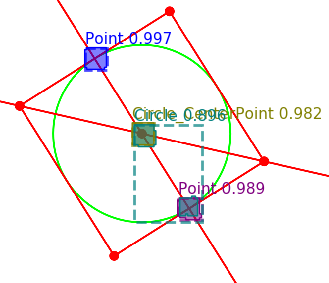
\includegraphics[width=100mm]{img/NO_POINT_DETECTION.png}
\caption{Example of the detection for level \textit{Alpha-10}, the goal of this level is to construct an incircle of a given square. The figure shows the current state of the construction (red), the remaining goal (green) and multiple detections of the Point Tool and Circle tool. The figure shows a potential problem if we do not use the automatic point detection (see Section \ref{no_point_detection}). If we do not use the automatic point detection, we have to detect usages of the Point tool as well. Then the network might prefer creating many points instead of using other tools.}
\label{no_point_detection_img}
\end{figure}

\begin{table}[t]
    \centering
    \begin{tabular}{| p{0.25\textwidth} | p{0.13\textwidth} | p{0.13\textwidth} | p{0.13\textwidth} | p{0.13\textwidth} |}%
    \hline
\multirow{2}{*}{\bfseries{Alpha levels}} &
\multicolumn{2}{m{0.3\textwidth}|}{\bfseries{without automatic point detection}} & \multicolumn{2}{m{0.3\textwidth}|}{\bfseries{automatic point detection}}
    \\
     & \bfseries Hints & \bfseries No hints & \bfseries Hints & \bfseries No hints
    \\\hline
    \csvreader[head to column names,late after line=\\, before filter=\ifthenelse{\equal{\csvcoli}{Accuracy}}{\csvfilterreject}{\csvfilteraccept}]{../img/tables/no_point_detection.csv}{}% use head of csv as column names
    {\level  & \PreviousHints & \Previous & \NoPointHints & \NoPoint}
    \hline
    \csvreader[head to column names, before filter=\ifthenelse{\equal{\csvcoli}{Accuracy}}{\csvfilteraccept}{\csvfilterreject}]{../img/tables/no_point_detection.csv}{}% use head of csv as column names
    {\bfseries{Average}  & \bfseries{\PreviousHints} & \bfseries{\Previous} & \bfseries{\NoPointHints} & \bfseries{\NoPoint}}
    \\\hline
    
    \end{tabular}
    \caption{Accuracy of Alpha levels during inference for the model with and without automatic point detection, evaluation on 500 instances for each level with and without hints. Note that some accuracies with hints can be slightly higher than without hints. Different permutations of construction steps can change the predictions of the model. When we use hints, we choose a prediction with the highest score that matches a hint, but there can be a higher score that does not match the hint.}
    \label{no_point_detection_table}
\end{table}

From Table \ref{no_point_detection_table} it is clear that automatic point detection improves the accuracy of every level. We can also see that automatic point detection no longer needs hints, as there is little difference between hint and no hints accuracy.
\subsection{History channel, more data on the input}
\label{history_channel}
Models generally have a problem to determine the exact step of the construction. We can observe that a single detection contains predictions of actions that correspond to actions used in later stages of the construction. In most cases, actions that are supposed to be used later have a lower Mask {R-CNN} score, but when they have a higher score, then we cannot solve the level by choosing only the top scoring hypothesis (see Section \ref{top_score_inference}). To avoid these situations, we add a history channel to the training data. With the current state in the first channel, the goal in the second channel, we add the previous state to the third channel. Furthermore, we can add a state before 2 steps to the fourth channel, a state before 3 steps to the fifth, and so on. However, we use only one history channel because we use the pre-trained Mask {R-CNN} model, and increasing the number of channels over 3 (over 1 history channel) we would have to train the whole Mask {R-CNN} model, including its backbone.

\begin{table}[th!]
    
    \begin{tabular}{| p{0.25\textwidth} | p{0.13\textwidth} | p{0.1\textwidth} |}%
    \hline
    \bfseries Alpha levels & \bfseries Without history & \bfseries With history
    \\\hline
    \csvreader[head to column names,late after line=\\,before filter=\ifthenelse{\equal{\csvcoli}{Accuracy}}{\csvfilterreject}{\csvfilteraccept}]{../img/tables/history_channel.csv}{}% use head of csv as column names
    {\level & \withouthistory & \withhistory}
    \hline
    \csvreader[head to column names, before filter=\ifthenelse{\equal{\csvcoli}{Accuracy}}{\csvfilteraccept}{\csvfilterreject}]{../img/tables/history_channel.csv}{}% use head of csv as column names
    {\bfseries{Average} & \bfseries{\withouthistory} & \bfseries{\withhistory}}
    \\\hline
    \end{tabular}
    \begin{tabular}{|p{0.25\textwidth} | p{0.1\textwidth} |}
         \hline
    \bfseries Beta levels & \bfseries With history
    \\ \hline
    \csvreader[head to column names,late after line=\\, before filter=\ifthenelse{\equal{\csvcoli}{Accuracy}}{\csvfilterreject}{\csvfilteraccept}]{../img/tables/history_channel.csv}{}% use head of csv as column names
    {\betalevel & \betawithhistory}
    \hline
    \csvreader[head to column names, before filter=\ifthenelse{\equal{\csvcoli}{Accuracy}}{\csvfilteraccept}{\csvfilterreject}]{../img/tables/history_channel.csv}{}% use head of csv as column names
    {\bfseries{Average} & \bfseries{\betawithhistory}}
    \\\hline
    \end{tabular}
    \caption{Accuracy of levels for the model with and without history (see Section \ref{history_channel}), evaluation on 500 instances for each level, for Alpha pack on the left and Beta pack on the right. Note that for Beta there is inference only with history. Model without history was not working on Beta at all. Models are based on the model with automatic point detection (see Section \ref{no_point_detection}).}
    \label{history_channel_table}
\end{table}

In Table \ref{history_channel_table} we can see an improvement of accuracy on the Alpha levels. Moreover, models with history were the first models that learned Beta levels with reasonable accuracy.
\newpage
\subsection{Stages of Mask {R-CNN}}
\label{stages_of_mercnn}
\begin{table}[h!]
    \centering
    \begin{tabular}{| p{0.25\textwidth} | p{0.13\textwidth} | p{0.08\textwidth} |}
    \hline
    \bfseries Beta levels & \bfseries Without 4+ & \bfseries With 4+ 
    \\\hline
    \csvreader[head to column names,late after line=\\, before filter=\ifthenelse{\equal{\csvcoli}{Accuracy}}{\csvfilterreject}{\csvfilteraccept}]{../img/tables/4plustraining.csv}{}% use head of csv as column names
    {\level & \previous & \fourplus }
    \hline
    \csvreader[head to column names, before filter=\ifthenelse{\equal{\csvcoli}{Accuracy}}{\csvfilteraccept}{\csvfilterreject}]{../img/tables/4plustraining.csv}{}% use head of csv as column names
    { \bfseries{Average} & \bfseries{\previous} & \bfseries{\fourplus} }
    \\\hline
    
    \end{tabular}
    \caption{Accuracy of levels during inference for models trained with the following setups. \textbf{Without 4+}: first 120 epochs training of head layers, then 80 epochs training the whole network. \textbf{With 4+}: first 60 epochs training of head layers, then 60 epochs of 4+ layers and then 80 epochs training the whole network. Both models have a history (see Section \ref{history_channel}), 500 instances of each level. Note that model without 4+ is the same model for Beta mentioned in Section \ref{history_channel_table}.}
    \label{four_plus_table}
\end{table}

Training of the Mask {R-CNN} is often divided into several stages. Each stage can have different training parameters. For training purposes, we have a stage with head layers, which are layers that compute masks from features detected in the backbone, and a stage with the backbone. The implementation of Mask {R-CNN} we use \cite{matterport_maskrcnn_2017} divides the backbone into multiple stages. It divides the backbone into 5 stages and allows to train only stages 3 and up, 4 and 5. We denote ``4+'' as training of the 4th and 5th stage of backbone and all head layers. Until now, we were using the following training setup: First, we train only head layers of Mask {R-CNN} and then we train the whole network. In Table \ref{four_plus_table} we can see the difference in accuracy if we include 4+ training, which shows that 4+ training improves accuracy on the beta level significantly. In Figure \ref{four_plus_losses} we can also see that models with 4+ training have a smoother loss. Spikes in epoch 60 and 120 are caused by enabling more layers to be trainable e.g.~first 60 epoch, we train only the head layer, and then we start 4+ as well. From epoch 120 we train the whole network.

\begin{figure}[h]
\centering
%models: logs/redoing_alpha/alpha_again_minimask ; logs/redoing_alpha/alpha_4+_included
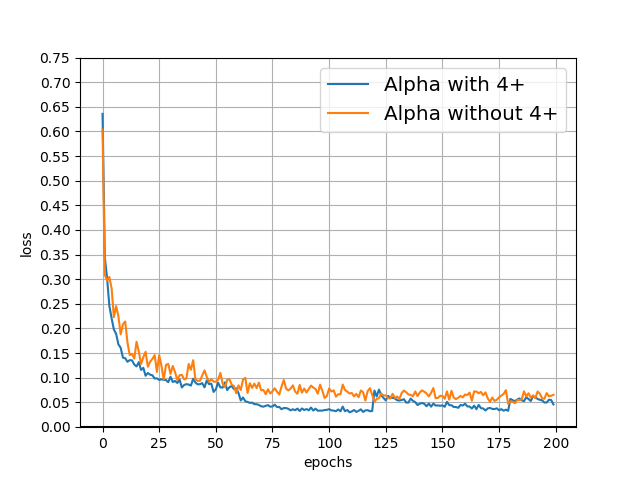
\includegraphics[width=140mm]{img/4+_losses.png}
\caption{Comparison of loss functions for training with and without 4+ training set-up (see Section \ref{stages_of_mercnn}). \textbf{Alpha without 4+} : epochs 0-120 training only heads, epochs 120-200 training the whole network. \textbf{Alpha with 4+} : epochs 0-60 training only heads, epochs 60-120 training only layers 4+ (i.e. backbone stages 4, 5 and the heads) and epochs 120-200 training the whole network. The loss for training with 4+ layers (blue) is much smoother and is less spiky than without 4+ (orange). }
\label{four_plus_losses}
\end{figure}

\subsection{Multiple solutions problem}

\begin{figure}[h!]
\centering
\begin{tabular}{ m{5cm} m{5cm}}
    \begin{subfigure}
    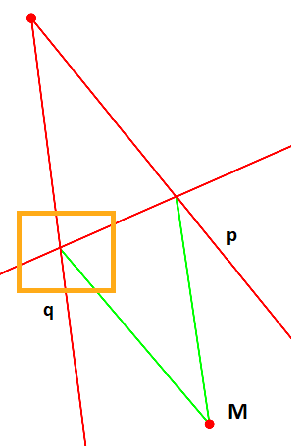
\includegraphics[width=47mm]{img/Gamma_gen_problem.png}
    \caption{}
    \label{gamma_close_dual_constr_main}
    \end{subfigure}
    &
    \begin{subfigure}
    \fbox{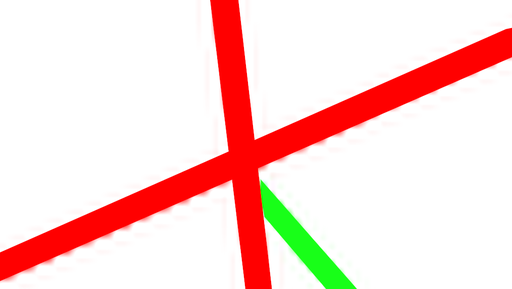
\includegraphics[width=47mm]{img/Gamma_gen_probem_detail.png}}
    \caption{detail of the orange area of Figure \ref{gamma_close_dual_constr_main}}
    \label{gamma_close_dual_constr_detail}
    \end{subfigure}
    \\
\end{tabular}
    
   
\caption{The degenerated instance of the level \text{Gamma-04}, the first step of the construction done. The goal is to find $X \in p, Y \in q$ such that $|MX| = |MY|$. Both solutions are very close to each other, and it is hard to recognize which solution we are supposed to construct. See detail in Figure \ref{gamma_close_dual_constr_detail}. Thus constructions are close as well. Hence the instance is degenerated. The degenerated configurations should not be in the training data nor in testing data because they are unsolvable based on image data.}
\label{gamma_close_dual_constr}
\end{figure}
To improve our generation process, we added the fourth degeneration rule: Intersections of geometric primitives can not be too close to the construction points (see Section \ref{degen_criteria}). The fourth rule was not applied to the data generation process while training and running inference for models in the sections above. Levels from Alpha and Beta packs are rarely considered as degenerated by the fourth rule. However, levels in the Gamma pack and above are. Some levels in Gamma are untrainable. Examples of these  are \textit{Gamma-04} and \textit{Gamma-05}. Around $27\%$ of \textit{Gamma-04} instances are considered as degenerated by the fourth rule while considered as valid by rules 1.~-3.~, in Figure \ref{gamma_close_dual_constr} we can see an example of this. This change allowed us to train Gamma and Delta levels. In Table \ref{new_gen_gamma_delta} we can see results if we add the fourth rule to the data generation. Level \textit{Delta-06}, construction of $\sqrt{2}$, has accuracy equal to $0$, because it is very similar to the \textit{Delta-07}, construction of $\sqrt{3}$, and models tend to prefer only one of these two levels. 


\begin{table}[h]
    \begin{tabular}{| p{0.28\textwidth} | p{0.15\textwidth} |}
    \hline
    \bfseries Gamma levels & \bfseries Accuracy 
    \\\hline
    \csvreader[head to column names,late after line=\\, before filter=\ifthenelse{\equal{\csvcoli}{Accuracy}}{\csvfilterreject}{
    \ifthenelse{\equal{\csvcoli}{}}{\csvfilterreject}{\csvfilteraccept}}]{../img/tables/gamma_delta_newgen.csv}{}% use head of csv as column names
    {\gammalevel & \gammaacc}
    \hline
    \csvreader[head to column names,late after line=\\, before filter=\ifthenelse{\equal{\csvcoli}{Accuracy}}{\csvfilteraccept}{\csvfilterreject}]{../img/tables/gamma_delta_newgen.csv}{}% use head of csv as column names
    { \bfseries{Average} & \bfseries{\gammaacc}}
    \hline
    
    \end{tabular} 
    \begin{tabular}{|p{0.28\textwidth} | p{0.15\textwidth} |}
        \hline
         \bfseries Delta levels & \bfseries Accuracy
         \\\hline
         \csvreader[head to column names,late after line=\\, before filter=\ifthenelse{\equal{\csvcoli}{Accuracy}}{\csvfilterreject}{\csvfilteraccept}]{../img/tables/gamma_delta_newgen.csv}{}% use head of csv as column names
        { \deltalevel & \deltaacc}
        \hline
        \csvreader[head to column names,late after line=\\, before filter=\ifthenelse{\equal{\csvcoli}{Accuracy}}{\csvfilteraccept}{\csvfilterreject}]{../img/tables/gamma_delta_newgen.csv}{}% use head of csv as column names
        { \bfseries{Average} & \bfseries{\deltaacc} }
        \hline
    \end{tabular}
    \caption{Accuracy of models for Gamma and Delta level packs for a new data generation. We include new degeneration rule: Intersections of geometric primitives can not be too close to the construction points (see (see Section \ref{degen_criteria}). Evaluation for Gamma level peck on the left and for the Delta level pack on the right. Note that the model with the fourth rule applied was the first model that was successfully able to solve Gamma and Delta level packs.}
    \label{new_gen_gamma_delta}
\end{table}
\subsection{On-the-fly generation}
\label{on_the_fly_section}
Until now, we were using pre-generated training data that had to be stored in memory. Pre-generated levels have to be in memory. Thus there is a limit to the size of the training data. The models described above contained 100 000 finished constructions of levels, the average length of construction is around 5 steps, thus 500 000 training examples had to be stored. To further increase the number of samples, we use generation on-the-fly, so each sample is seen only once during the training. Keep in mind that history, degeneration checks, and multi-thread training have to be adjusted as well. In Figure \ref{on_the_fly_gen_loss}
we can make a comparison of losses for models using pre-generated and on-the-fly generation. The loss of the model with on-the-fly generation decreases at a lower rate. However, the loss function is smoother, and the model achieves better accuracy during inference. The accuracy is equal to $0.991$, compared to $0.735$ accuracy of the model with a pre-generated dataset. Although a model with on-the-fly generation has a higher loss value, it generalizes better due to the variety of the training data, e.g.~the model with pre-generated data is prone to over-fitting.
\begin{figure}[h]
\centering
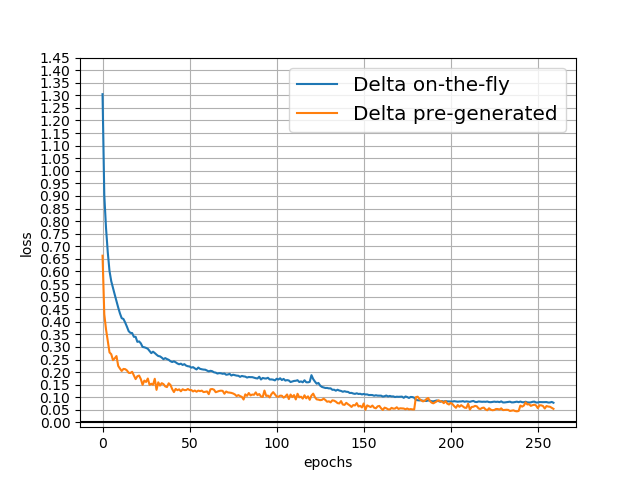
\includegraphics[width=\textwidth]{img/on-the-fly-gen.png}
\caption{Loss of models that uses 500k pre-generated training examples (Delta pre-generated) and 3.2M training examples generated on-the-fly (Delta on-the-fly).  Both networks were trained in the following setup: epochs 0-60 training only heads, epochs 60-120 training only layers 4+ (i.e. backbone stages 4, 5 and the heads) and epochs 120-200 training the whole network. Note that pre-generated training data are forwarded in the network with in a random order, but samples generated on-the-fly are fed to the network in the order they were created.}
\label{on_the_fly_gen_loss}
\end{figure}
\section{Evaluation of supervised learning approach}
\label{supervised_evaluation}
With components described in the previous Section \ref{design_choices}, we can train models that can solve entire packs or even multiple packs at once. We evaluate models on the first six level packs (Alpha, Beta, Gamma, Delta, Epsilon, Zeta). All those packs are prepared for data generation, and thus to training. 
\newline \newline
We trained a model for each level (68) for the first 6 level packs of Euclidea. Each model is trained for 200 epochs. Each epoch consists of 16~000 training samples, e.g.~1~000 training steps of batches of size 16. The model generates data on-the-fly (see Section \ref{on_the_fly_section}). Hence $3.2M$ training samples are seen during the training. In the first 120 epochs, we train only head layers, then 60 epochs of 4+ layers and the last 60 epochs train the whole network (see Section \ref{stages_of_mercnn}). Initial weights of the model are weights from the COCO model, which is part of Matterport \cite{matterport_maskrcnn_2017}. This model has an average $97.7\%$ accuracy, which has been evaluated on 500 instances for each level in Alpha to Zeta packs. Results are summarized in Table \ref{final_model_results}.
\newline \newline
We also trained single model for each level pack. Models for level packs are trained in the same way, and the only difference is the number of epochs. Level pack models are trained for 260 epochs: 120 heads, 60 epochs of 4+ and 80 epochs of the whole network. Level pack models have the following accuracies reported in Table \ref{final_model_results}.
\newline \newline
Finally, we trained a single model for all levels. The training setup of this model is the same as for individual models and level pack models. The only difference is the number of epochs. The model was trained for 400 epochs ($6.4M$ training samples): 200 heads, 100 of 4+ and 100 of the whole network. This model has an average $91.8\%$ accuracy and the hypothesis tree search accuracy of $92.1\%$. Accuracies for each level are in Appendix \ref{all_model_tree_search}).
\newline \newline
\begin{table}[h]
\begin{tabular}{l| l l l l l l}
Model / Level Pack & Alpha & Beta & Gamma & Delta & Epsilon & Zeta
 \\ \hline
 one model per level & $98.7\%$ & $98.6\%$ & $97.4\%$ & $99.3\%$ & $96.3\%$ & $96.0\%$\\
 one model per pack & $96.1\%$& $96.2\%$ & $97.8\%$& $99.1\%$ & $92.8\%$ & $95.7\%$ \\
 one model for all levels & $90.0\%$ & $94.4\%$ & $89.4\%$ & $96.9\%$ & $88.6\%$ & $91.5\%$ \\
 \end{tabular}
 \caption{Final results of models for all levels, level packs and individual models. Each column represents the average accuracy of the model(s) on all levels (500 instances for each level) of a respective pack. \textbf{Individual models}: One model for each of 68 levels, accuracy is measured only for a model on a corresponding level. \textbf{level pack models}: One model for each of 6 level packs. Inference of the pack measured for a model trained for a respective pack. \textbf{all level model}: One model is used for all levels.}
 \label{final_model_results}
\end{table}

\section{Evaluation of supervised learning on unseen problems
}
\label{eval_of_unseen_levels}
To evaluate a model's performance on unseen levels, we use the leave-one-out method with the hypothesis tree search (see Sections \ref{hypotheses_tree_search} and \ref{leave_one_out_method}).  We use models for all levels and all level packs from the previous chapter. The results are shown in Figures \ref{leave_one_out_levels} and \ref{leave_one_out_packs} we can see results of the leave-one-out evaluation of hypothesis tree search. Some levels can be solved this way, but others cannot. To solve an unseen level, we have to have parts of the construction in models we have seen in training, e.g.~ the first part of the construction can be done with a model X and the second part with a model Y.
\begin{table}[ht]
    \centering
    \begin{tabular}{ p{0.30\textwidth}  p{0.15\textwidth}  p{0.45\textwidth}}
    %\hline
    \bfseries Level & \bfseries Accuracy & \bfseries Connections
    % \hline
    \end{tabular}
    \vspace*{2mm}
    \textbf{Alpha}
    \begin{tabular}{ p{0.30\textwidth}  p{0.15\textwidth} p{0.45\textwidth}}
    \hline
    %\bfseries Level & \bfseries Accuracy & \bfseries Connections
    \csvreader[head to column names,separator=semicolon
    ]{../img/tables/leave_one_out_levels_alpha.csv}{}% use head of csv as 
    {\\[0.05cm]\level & \accuracy & \connections}
    \end{tabular}
    \textbf{Beta}
    \begin{tabular}{ p{0.30\textwidth}  p{0.15\textwidth}  p{0.45\textwidth}}
    \hline
    \csvreader[head to column names,separator=semicolon ]{../img/tables/leave_one_out_levels_beta.csv}{}% use head of csv as 
    {\\[0.05cm]\level & \accuracy & \connections}
    %\hline
    \end{tabular}
    \textbf{Gamma}
    \begin{tabular}{ p{0.30\textwidth}  p{0.15\textwidth}  p{0.45\textwidth}}
    \hline
    \csvreader[head to column names,separator=semicolon ]{../img/tables/leave_one_out_levels_gamma.csv}{}% use head of csv as 
    {\\[0.05cm]\level & \accuracy & \connections}
    %\hline
    \end{tabular}
    \textbf{Epsilon}
    \begin{tabular}{ p{0.30\textwidth}  p{0.15\textwidth} 
    p{0.45\textwidth}}
    \hline
    \csvreader[head to column names,separator=semicolon ]{../img/tables/leave_one_out_levels_epsilon.csv}{}% use head of csv as 
    {\\[0.05cm]\level & \accuracy & \connections}
    %\hline
    \end{tabular}
    \textbf{Zeta}
    \begin{tabular}{p{0.30\textwidth}  p{0.15\textwidth}  p{0.45\textwidth}}
    \hline
    \csvreader[head to column names,separator=semicolon ]{../img/tables/leave_one_out_levels_zeta.csv}{}% use head of csv as 
    {\\[0.05cm]\level & \accuracy & \connections}
    \\
    \end{tabular}
    
    
   \caption{Leave-one-out evaluation of hypothesis tree search for each level pack. Model for \textbf{each level} within a pack are inputs for the method, e.g.~accuracy on Alpha-01 with other Alpha models and so on. Note that 38 not solved levels are not shown in the table, remaining 30 levels are present in the table. Connected levels contribute to a solutions of other levels (see Section \ref{connections}).}
    \label{leave_one_out_levels}
\end{table}
\begin{table}[ht]
    \centering
    \begin{tabular}{ p{0.30\textwidth}  p{0.15\textwidth}  p{0.45\textwidth}}
    %\hline
    \bfseries Level & \bfseries Accuracy & \bfseries Connections
    % \hline
    \end{tabular}
    \textbf{Alpha}
    \begin{tabular}{ p{0.30\textwidth}  p{0.15\textwidth} p{0.45\textwidth}}
    \hline
    %\bfseries Level & \bfseries Accuracy & \bfseries Connections
    \csvreader[head to column names,separator=semicolon, before filter=\ifthenelse{\equal{\csvcolii}{0.00}}{\csvfilterreject}{\csvfilteraccept} ]{../img/tables/leave_one_out_pack_alpha.csv}{}% use head of csv as 
    {\\[0.05cm]\level & \accuracy & \connections}
    %\hline
    \end{tabular}
    \textbf{Beta}
    \begin{tabular}{ p{0.30\textwidth}  p{0.15\textwidth}  p{0.45\textwidth}}
    \hline
    \csvreader[head to column names,separator=semicolon, before filter=\ifthenelse{\equal{\csvcolii}{0.00}}{\csvfilterreject}{\csvfilteraccept}  ]{../img/tables/leave_one_out_pack_beta.csv}{}% use head of csv as 
    {\\[0.05cm]\level & \accuracy & \connections}
    %\hline
    \end{tabular}
    \textbf{Gamma}
    \begin{tabular}{ p{0.30\textwidth}  p{0.15\textwidth}  p{0.45\textwidth}}
    \hline
    \csvreader[head to column names,separator=semicolon, before filter=\ifthenelse{\equal{\csvcolii}{0.00}}{\csvfilterreject}{\csvfilteraccept}  ]{../img/tables/leave_one_out_pack_gamma.csv}{}% use head of csv as 
    {\\[0.05cm]\level & \accuracy & \connections}
    %\hline
    \end{tabular}
    \textbf{Epsilon}
    \hline
    \begin{tabular}{ p{0.30\textwidth}  p{0.15\textwidth}  p{0.45\textwidth}}
    \csvreader[head to column names,separator=semicolon, before filter=\ifthenelse{\equal{\csvcolii}{0.00}}{\csvfilterreject}{\csvfilteraccept}  ]{../img/tables/leave_one_out_pack_epsilon.csv}{}% use head of csv as 
    {\\[0.05cm]\level & \accuracy & \connections}
    %\hline
    \end{tabular}
    \textbf{Zeta}
    \hline
    \begin{tabular}{ p{0.30\textwidth}  p{0.15\textwidth}  p{0.45\textwidth}}
    \csvreader[head to column names,separator=semicolon, before filter=\ifthenelse{\equal{\csvcolii}{0.00}}{\csvfilterreject}{\csvfilteraccept}  ]{../img/tables/leave_one_out_pack_zeta.csv}{}% use head of csv as 
    {\\[0.05cm]\level & \accuracy & \connections}
    %\hline
    \end{tabular}
    
    
    \caption{Leave-one-out evaluation of hypothesis tree search for each level pack. Model for \textbf{each pack} are inputs for the method, e.g.~accuracy on Alpha with models for Beta-Zeta and so on. Note that 37 not solved levels are not shown in the table, remaining 31 levels are present in the table. Connected levels contribute to a solutions of other levels (see Section \ref{connections}).}
    \label{leave_one_out_packs}
\end{table}


\section{Example results}
\label{example_of_level}
In this section, we show Tables with detailed walk-through of constructions for levels \textit{Gamma-08} in \ref{Gamma08_example}, \textit{Delta-10} in \ref{Delta10_example} and \textit{Epsilon-12} in \ref{Epsilon12_example}. For each inference, we use a single model trained on all 68 levels from Alpha to Zeta.
\subsection{Gamma 08 - lozenge}
\begin{longtable}[h]{p{7cm}p{7.25cm}}
\subfloat{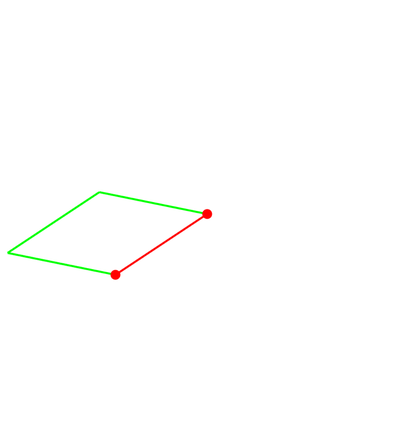
\includegraphics[scale=0.4]{img/Gamma-08_example/input_image0.png}} &
\subfloat{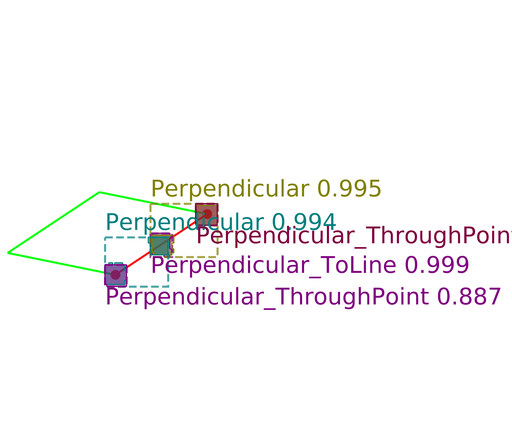
\includegraphics[scale=0.4]{img/Gamma-08_example/output_image0.png}}\\

a) Level definition and first input for the network. The goal of this level is to construct a rhombus with a given side and angle of $45^\circ$ in a vertex. The green color denotes the goal and the red denotes the current state of the construction.& 
b) Prediction of the network. We can see there are two predictions of the Perpendicular tool. Both can be used, but the top one has a slightly higher Mask {R-CNN} score.\\

\subfloat{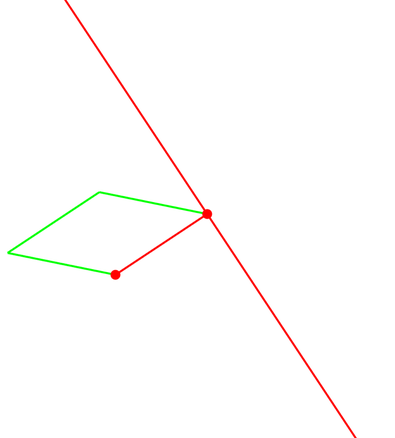
\includegraphics[scale=0.4]{img/Gamma-08_example/input_image1.png}} &
\subfloat{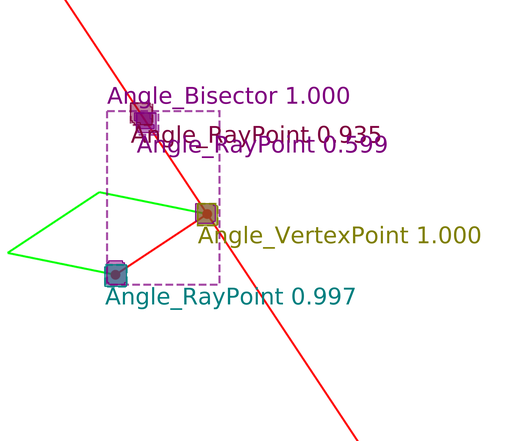
\includegraphics[scale=0.4]{img/Gamma-08_example/output_image1.png}}\\

c) Step 1. &
d) Prediction for step 2. Based on this prediction, an angle bisector will be constructed. Note that there are multiple Angle ray points on the top ray (purple). Either of them can be used with the same result.\\

\subfloat{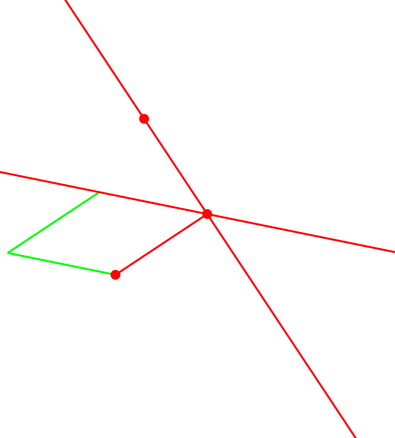
\includegraphics[scale=0.4]{img/Gamma-08_example/input_image2.png}} &
\subfloat{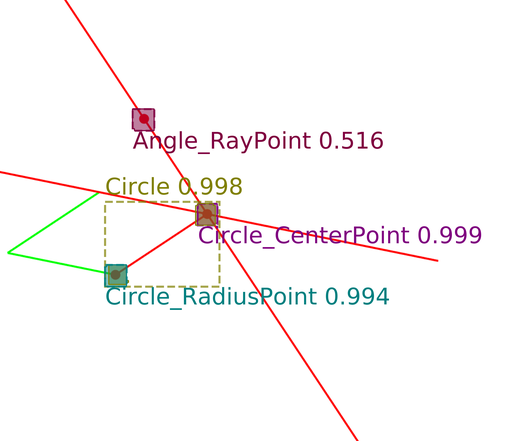
\includegraphics[scale=0.4  ]{img/Gamma-08_example/output_image2.png}}\\

e) Step 2. Last step constructed part of the goal, one side of the rhombus.& 
f) Prediction for step 3. Based on this prediction, a circle will be constructed.\\

\subfloat{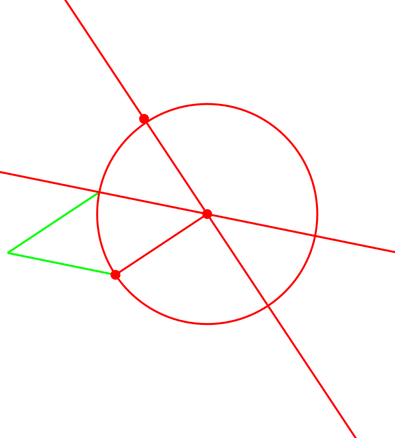
\includegraphics[scale=0.4  ]{img/Gamma-08_example/input_image3.png}} &
\subfloat{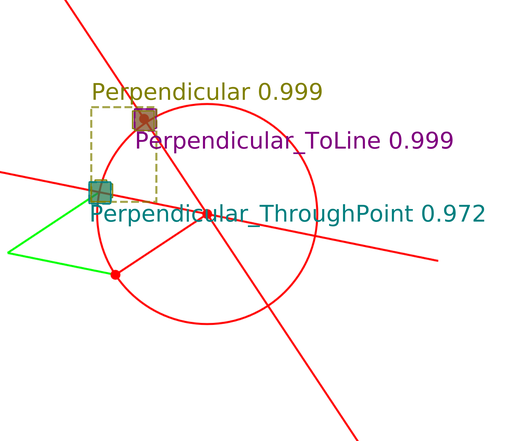
\includegraphics[scale=0.4  ]{img/Gamma-08_example/output_image3.png}}\\

g) Step 3. Note that the point at the top does not lie on the constructed circle.
& h) Prediction for step 4. Based on this prediction, a perpendicular line will be constructed.\\

\subfloat{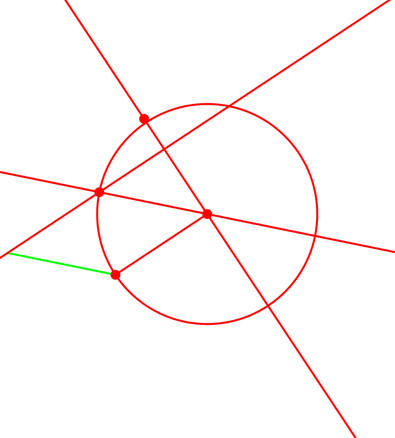
\includegraphics[scale=0.4  ]{img/Gamma-08_example/input_image4.png}} &
\subfloat{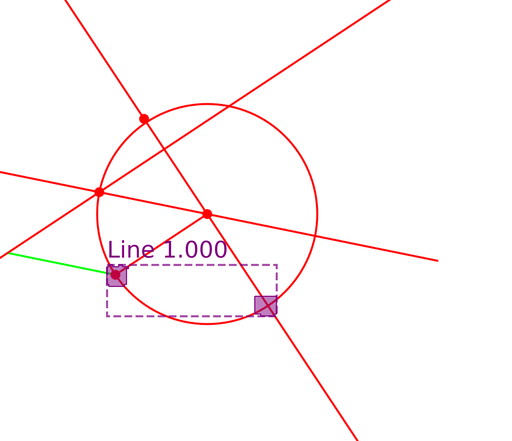
\includegraphics[scale=0.4  ]{img/Gamma-08_example/output_image4.png}}\\

i) Step 4. The last perpendicular constructed another part of the goal.
& j) Prediction for step 5. Based on this prediction, a line will be constructed.\\

\subfloat{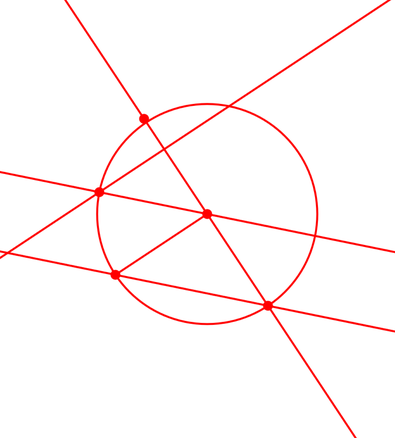
\includegraphics[scale=0.4  ]{img/Gamma-08_example/input_image5.png}}\\
k) step 7 - level successfully finished, all goals are constructed.\\
    \caption{Example of construction of level \textit{Gamma-08}: Lozenge. The goal of this level is to construct a rhombus with a given side and angle of $45^\circ$ in a vertex. The table contains all construction steps of the level. Each step contains current progress on the left and Mask {R-CNN} prediction for a new step on the right. The green color denotes the goal and the red denotes the current state of the construction. Other colors mark prediction masks, bounding boxes, classes and scores for each detected object.}
    \label{Gamma08_example}
\end{longtable}
\subsection{Delta 10 - square by adjacent midpoints}
\begin{longtable}[h]{p{7.25cm}p{7.25cm}}
\subfloat{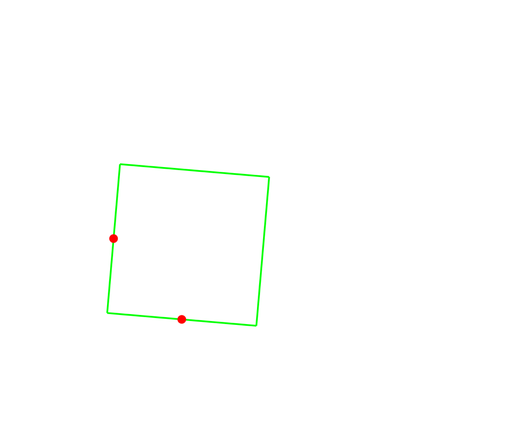
\includegraphics[scale=0.4]{img/Delta-10_example/input_image0.png}} &
\subfloat{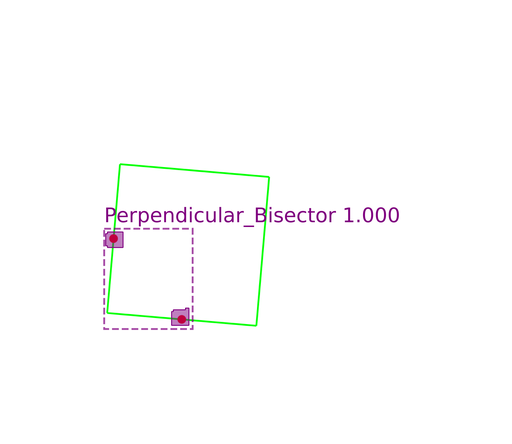
\includegraphics[scale=0.4]{img/Delta-10_example/output_image0.png}}\\

a) Level definition and first input for the network. Construct a square by adjacent side midpoints. The green color denotes the goal and the red denotes the current state of the construction.& 
b) Prediction of the network, perpendicular bisector.\\

\subfloat{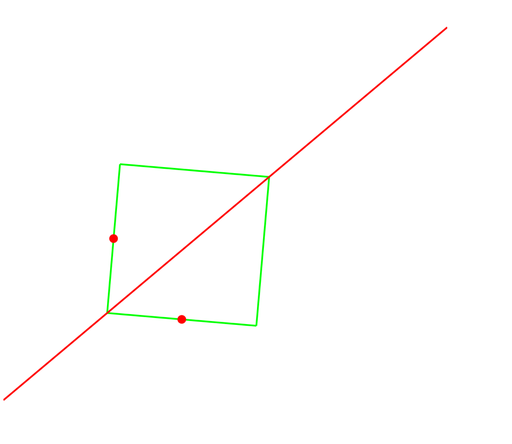
\includegraphics[scale=0.4]{img/Delta-10_example/input_image1.png}} &
\subfloat{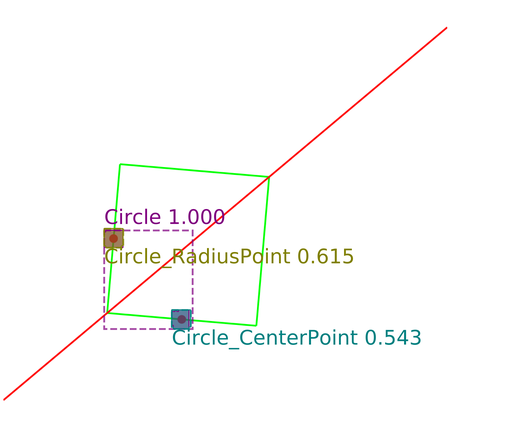
\includegraphics[scale=0.4]{img/Delta-10_example/output_image1.png}}\\

c) Step 1. &
d) Prediction for step 2. Based on this prediction, a circle will be constructed.\\

\subfloat{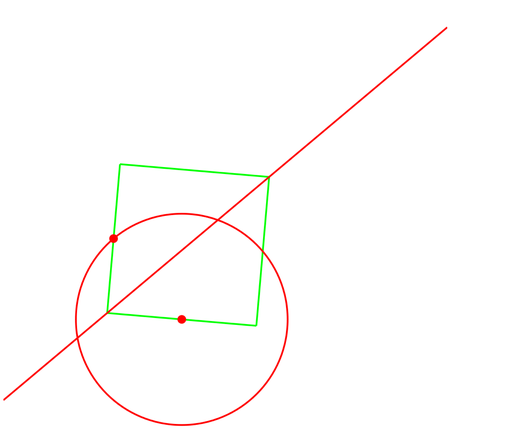
\includegraphics[scale=0.4]{img/Delta-10_example/input_image2.png}} &
\subfloat{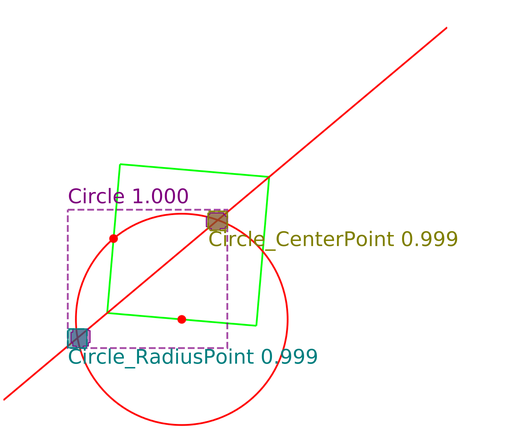
\includegraphics[scale=0.4  ]{img/Delta-10_example/output_image2.png}}\\

e) Step 2.& 
f) Prediction for step 3. Based on this prediction, a circle will be constructed.\\

\subfloat{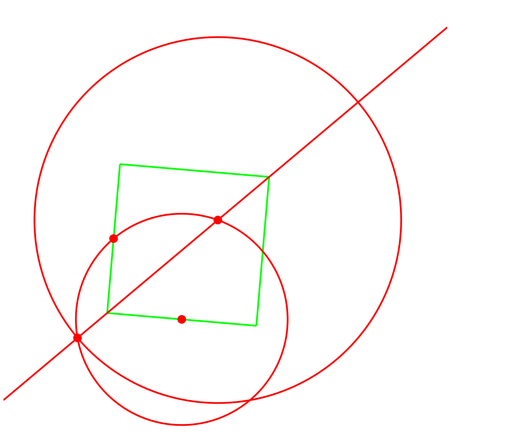
\includegraphics[scale=0.4  ]{img/Delta-10_example/input_image3.png}} &
\subfloat{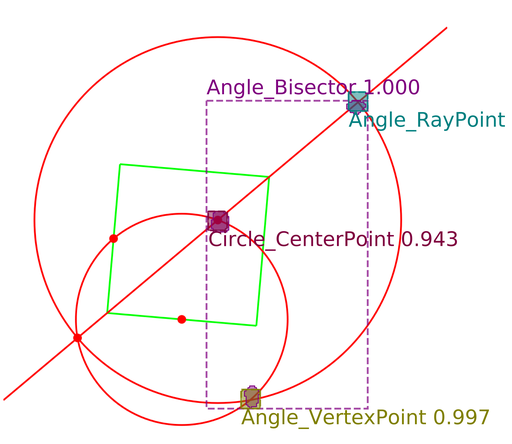
\includegraphics[scale=0.4  ]{img/Delta-10_example/output_image3.png}}\\

g) Step 3. 
& h) Prediction for step 4. Based on this prediction, an angle bisector  will be constructed. Note that one ray point is not marked with detection, instead it is marked with the circle center point detection, which is a mistake. This prediction should be in the previous step. However, our model is still able to recognize all points to execute the Angle Bisector tool .\\

\subfloat{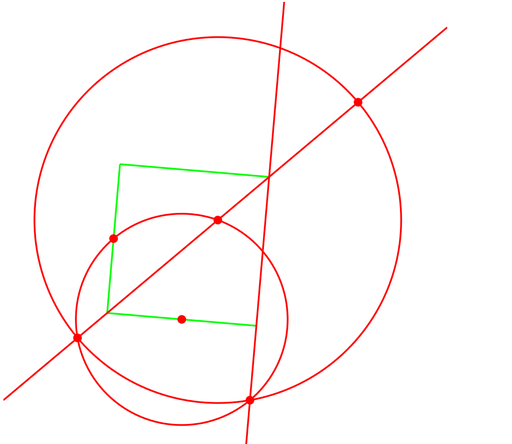
\includegraphics[scale=0.4  ]{img/Delta-10_example/input_image4.png}} &
\subfloat{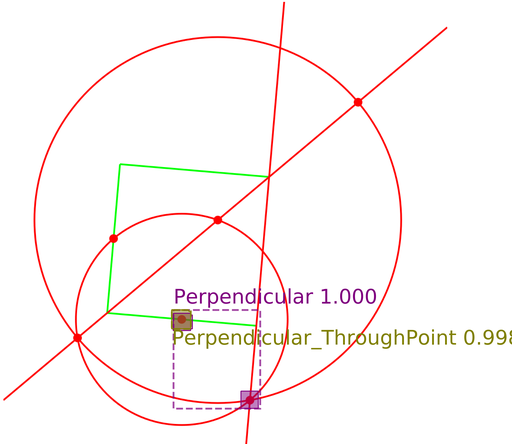
\includegraphics[scale=0.4  ]{img/Delta-10_example/output_image4.png}}\\

i) Step 4. The last angle bisector constructed part of the goal.
& j) Prediction for step 5. Based on this prediction, a perpendicular line  will be constructed.\\

\subfloat{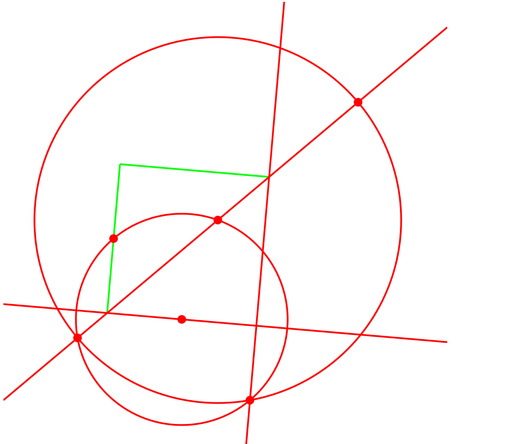
\includegraphics[scale=0.4  ]{img/Delta-10_example/input_image5.png}} &
\subfloat{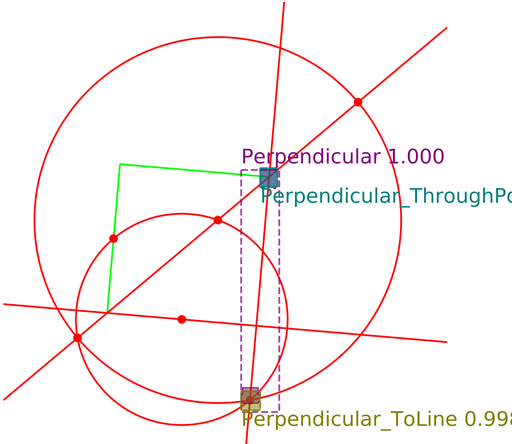
\includegraphics[scale=0.4  ]{img/Delta-10_example/output_image5.png}}\\

l) Step 5. The last perpendicular constructed another part of the goal.
& l) Prediction for step 5. Based on this prediction, a perpendicular line  will be constructed.\\

\subfloat{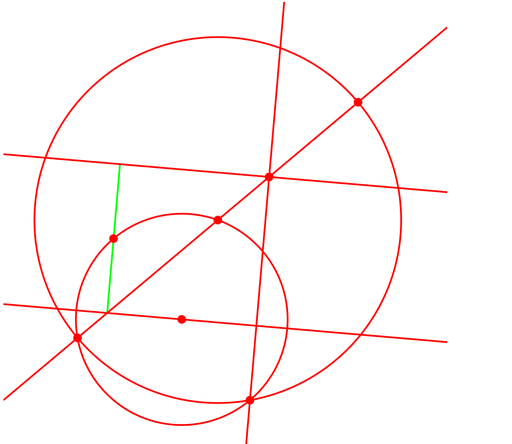
\includegraphics[scale=0.4  ]{img/Delta-10_example/input_image6.png}} &
\subfloat{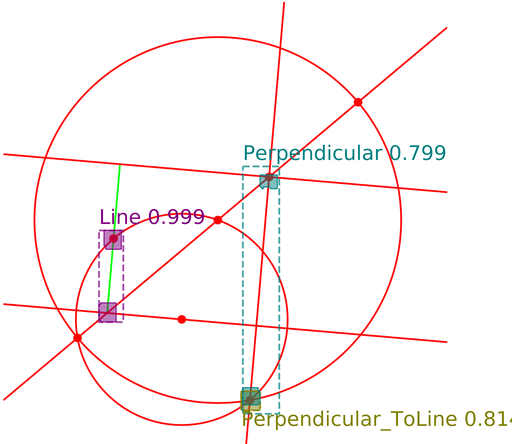
\includegraphics[scale=0.4  ]{img/Delta-10_example/output_image6.png}}\\

m) Step 6. The last perpendicular constructed another part of the goal.
& n) Prediction for step 5. Based on this prediction, a perpendicular line  will be constructed.\\

\subfloat{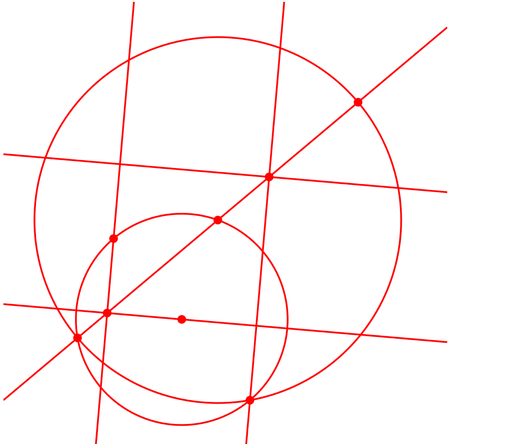
\includegraphics[scale=0.4  ]{img/Delta-10_example/input_image7.png}}\\
o) step 7 - level successfully finished, all goals are constructed.\\


\caption{Example of construction of level \textit{Delta-10}: Square by adjacent side midpoints. The table contains all construction steps of the level. Each step contains current progress on the left and Mask {R-CNN} prediction for a new step on the right. The green color denotes the goal and the red denotes the current state of the construction. Other colors mark prediction masks, bounding boxes, classes and scores for each detected object.}
\label{Delta10_example}
\end{longtable}
\subsection{Epsilon 12 - regular hexagon by the side}
\begin{longtable}[h]{p{7.25cm}p{7.25cm}}
\subfloat{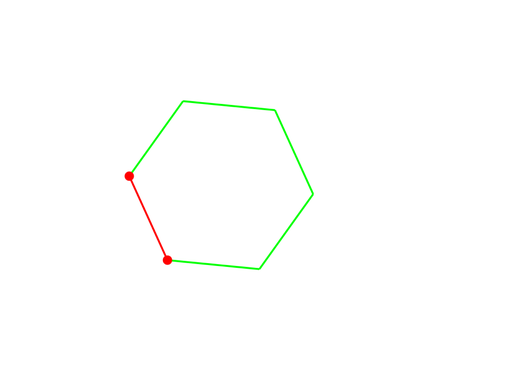
\includegraphics[scale=0.4]{img/Epsilon-12_example/input_image0.png}} &
\subfloat{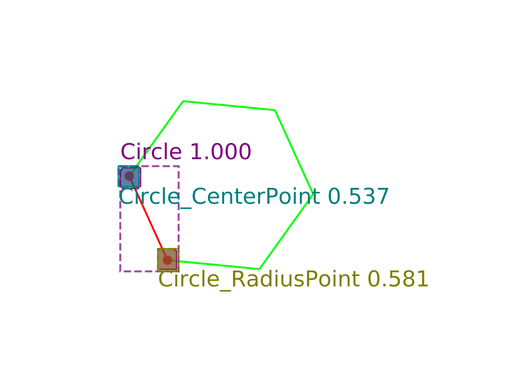
\includegraphics[scale=0.4]{img/Epsilon-12_example/output_image0.png}}\\

a) Level definition and first input for the network. Construct a regular hexagon given by the side. The green color denotes the goal and the red denotes the current state of the construction. & 
b) Prediction of the network.Based on this prediction, a circle will be constructed.\\

\subfloat{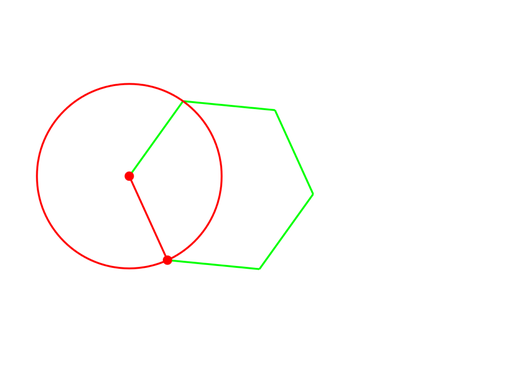
\includegraphics[scale=0.4]{img/Epsilon-12_example/input_image1.png}} &
\subfloat{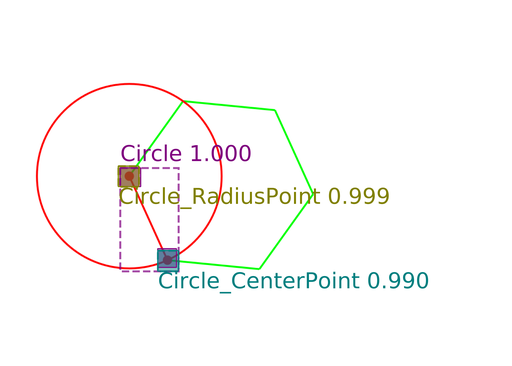
\includegraphics[scale=0.4]{img/Epsilon-12_example/output_image1.png}}\\

c) Step 1. &
d) Prediction for step 2. Based on this prediction, a line will be constructed.\\

\subfloat{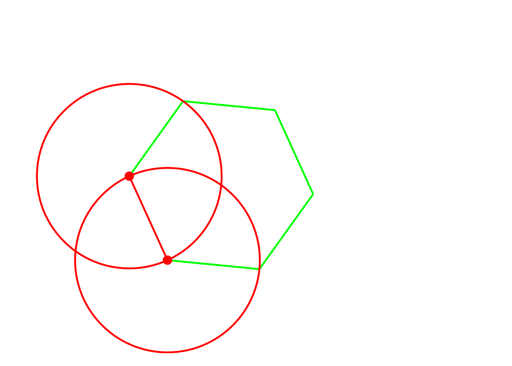
\includegraphics[scale=0.4]{img/Epsilon-12_example/input_image2.png}} &
\subfloat{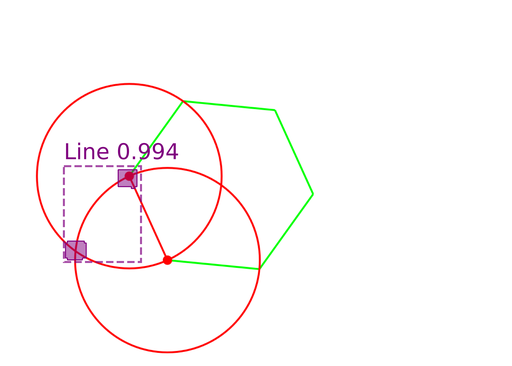
\includegraphics[scale=0.4  ]{img/Epsilon-12_example/output_image2.png}}\\

e) Step 2.& 
f) Prediction for step 3. Based on this prediction, a line will be constructed.\\

\subfloat{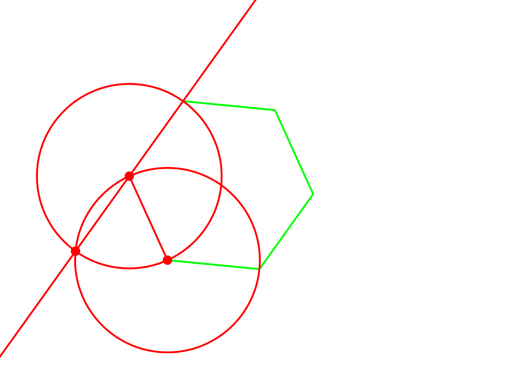
\includegraphics[scale=0.4  ]{img/Epsilon-12_example/input_image3.png}} &
\subfloat{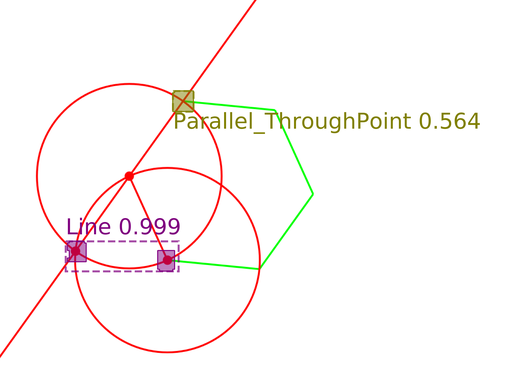
\includegraphics[scale=0.4  ]{img/Epsilon-12_example/output_image3.png}}\\

g) Step 3. 
& h) Prediction for step 4. Based on this prediction, an angle bisector will be constructed. Note that there is an extra detection of parallel through point. Later in construction score of this prediction will increase and the prediction will be used.\\

\subfloat{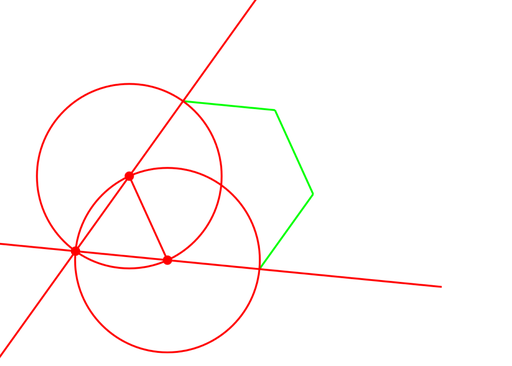
\includegraphics[scale=0.4  ]{img/Epsilon-12_example/input_image4.png}} &
\subfloat{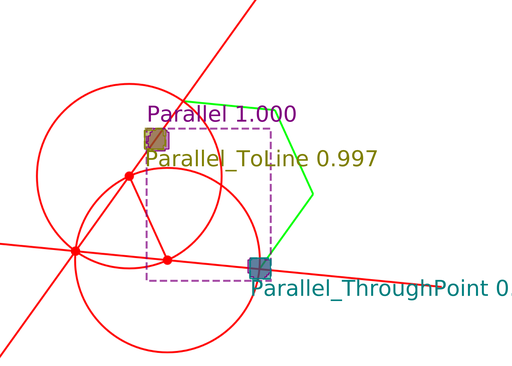
\includegraphics[scale=0.4  ]{img/Epsilon-12_example/output_image4.png}}\\

i) Step 4. The last parallel line constructed part of the goal.
& j) Prediction for step 5. Based on this prediction, a parallel line will be constructed.\\

\subfloat{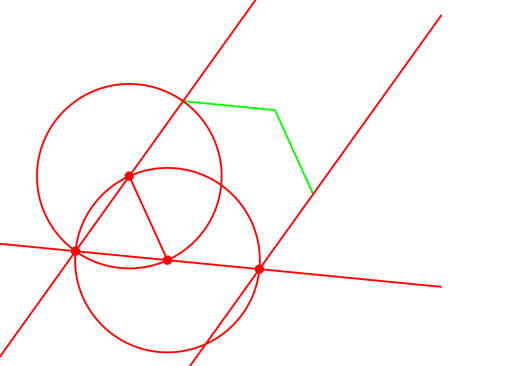
\includegraphics[scale=0.4  ]{img/Epsilon-12_example/input_image5.png}} &
\subfloat{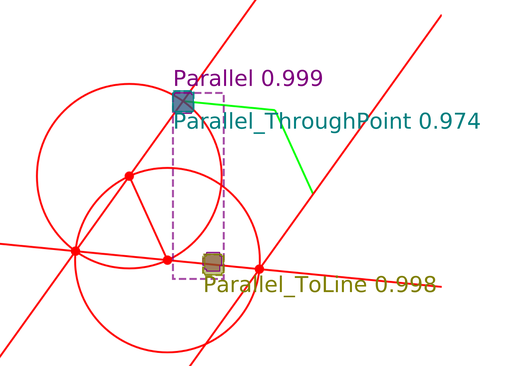
\includegraphics[scale=0.4  ]{img/Epsilon-12_example/output_image5.png}}\\

l) Step 5. The last parallel line constructed another part of the goal.
& l) Prediction for step 5. Based on this prediction, a parallel line will be constructed.\\

\subfloat{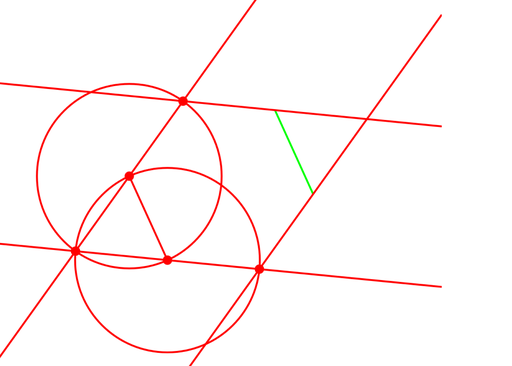
\includegraphics[scale=0.4  ]{img/Epsilon-12_example/input_image6.png}} &
\subfloat{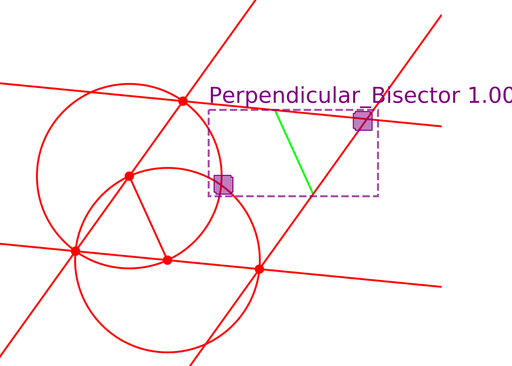
\includegraphics[scale=0.4  ]{img/Epsilon-12_example/output_image6.png}}\\

m) Step 6. The last perpendicular bisector constructed another part of the goal.
& n) Prediction for step 5. Based on this prediction, a perpendicular bisector will be constructed.\\

\subfloat{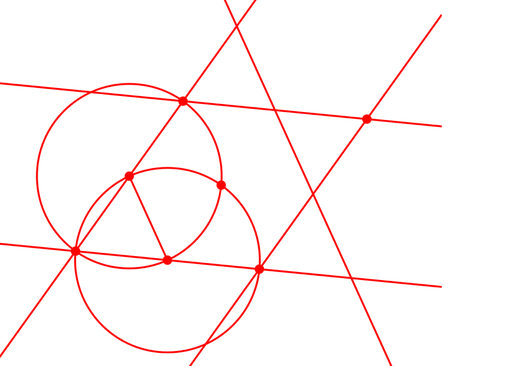
\includegraphics[scale=0.4  ]{img/Epsilon-12_example/input_image7.png}}\\
o) step 7 - level successfully finished, all goals are constructed.\\


\caption{Example of construction of level \textit{Epsilon-12}: regular hexagon by the side. The table contains all construction steps of the level. Each step contains current progress on the left and Mask {R-CNN} prediction for a new step on the right. The green color denotes the goal and the red denotes the current state of the construction. Other colors mark prediction masks, bounding boxes, classes and scores for each detected object.}
\label{Epsilon12_example}
\end{longtable}